\section{PDE 与 PTE 位域格式}

PDE 和 PTE 共享相同的 32 位格式，仅 bit 6--7 的含义略有区别：

\begin{figure}[H]
  \centering
  % figures/ch08/fig03-pde-pte-bits.tex — auto-extracted from chapter source
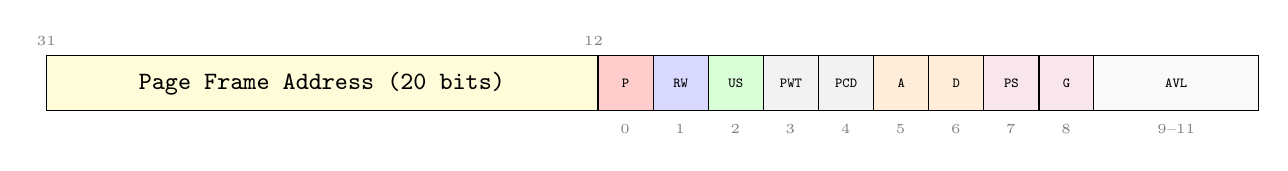
\begin{tikzpicture}[
  bitcell/.style={draw, minimum width=0.7cm, minimum height=0.7cm, font=\ttfamily\tiny, anchor=west},
  bitlabel/.style={font=\tiny, text=gray},
]
  % 高 20 位 — 页帧地址
  \node[draw, minimum width=7cm, minimum height=0.7cm, fill=yellow!15, font=\small\ttfamily]
    (frame) at (0, 0) {Page Frame Address (20 bits)};
  \node[bitlabel, above] at (-3.5, 0.35) {31};
  \node[bitlabel, above] at (3.45, 0.35) {12};

  % 低 12 位 — flags
  \foreach \i/\txt/\col in {
    0/P/red!20,
    1/R\/W/blue!15,
    2/U\/S/green!15,
    3/PWT/gray!10,
    4/PCD/gray!10,
    5/A/orange!15,
    6/D/orange!15,
    7/PS/purple!10,
    8/G/purple!10
  } {
    \node[bitcell, fill=\col] (b\i) at (3.5+\i*0.7, 0) {\txt};
  }
  % AVL bits 9-11
  \node[draw, minimum width=2.1cm, minimum height=0.7cm, fill=gray!5, font=\ttfamily\tiny]
    (avl) at (9.8+1.05, 0) {AVL};

  % bit 标注
  \foreach \i/\b in {0/0, 1/1, 2/2, 3/3, 4/4, 5/5, 6/6, 7/7, 8/8} {
    \node[bitlabel, below] at (3.5+\i*0.7+0.35, -0.4) {\b};
  }
  \node[bitlabel, below] at (10.85, -0.4) {9--11};
\end{tikzpicture}

  \caption{PDE/PTE 32 位格式}
  \label{fig:pde-pte-bits}
\end{figure}

\begin{longtable}{clp{8.5cm}}
  \toprule
  \textbf{Bit} & \textbf{名称} & \textbf{说明} \\
  \midrule
  0 & P (Present) & 1 = 条目有效；0 = 访问触发 \#PF (Page Fault) \\
  1 & R/W & 1 = 可读写；0 = 只读 \\
  2 & U/S & 1 = Ring\,3 可访问；0 = 仅 Ring\,0 \\
  3 & PWT & Write-Through 缓存策略（通常置 0） \\
  4 & PCD & Cache Disable（通常置 0） \\
  5 & A (Accessed) & CPU 访问此页后自动置 1 \\
  6 & D (Dirty) & CPU 写入此页后自动置 1（PTE 有意义） \\
  7 & PS/PAT & PDE: PS=1 启用 4\,MiB 大页；PTE: PAT 位 \\
  8 & G (Global) & 1 = TLB 不随 CR3 切换刷新（需 \reg{CR4}.PGE） \\
  9--11 & AVL & 软件可用（OS 自定义用途） \\
  12--31 & Frame & 物理页帧地址的高 20 位（低 12 位隐含为 0，即 4\,KiB 对齐） \\
  \bottomrule
\end{longtable}

我们的内核目前只用到三个 flag 宏：

\codefile{src/include/kernel/vmm.h}
\begin{lstlisting}[style=cstyle]
#define PTE_PRESENT     0x001u  /* bit 0: 条目有效 */
#define PTE_WRITABLE    0x002u  /* bit 1: 可读写   */
#define PTE_USER        0x004u  /* bit 2: 用户态可访问 */

#define PDE_PRESENT     0x001u
#define PDE_WRITABLE    0x002u
#define PDE_USER        0x004u
\end{lstlisting}

\begin{designbox}
PDE flags 遵循"宽松上限"原则：PDE 给足权限（Present + Writable），
精细控制放在 PTE 层。例如 PDE 设 Writable 但 PTE 设 Read-Only，最终该页只读；
反之 PDE 设 Read-Only，即使 PTE 设 Writable，该页也只读。所以我们
在 PDE 层统一设 \texttt{PDE\_PRESENT | PDE\_WRITABLE}，
具体的只读/用户态权限在 PTE 中控制。
\end{designbox}

% ============================================================================

